\documentclass{article}
\usepackage[UTF8]{ctex}
\usepackage[T1]{fontenc}
\usepackage[utf8]{inputenc}
\usepackage{float}
\usepackage{placeins}
\usepackage{latexsym}
\usepackage{amsmath}
\usepackage{amsthm}
\usepackage{amssymb}
\usepackage{listings}
\usepackage{xcolor}
\usepackage{ulem}
\usepackage{multicol}
\usepackage{geometry}
\usepackage{hyperref}
\usepackage{tikz}
\usetikzlibrary{positioning}
\usetikzlibrary[arrows, shapes, chains]
\hypersetup{
	colorlinks=true,
	urlcolor=black,
}
\lstset
{
    basicstyle = \ttfamily,
    keywordstyle = \bfseries\color{blue!70},
    commentstyle = \songti \upshape,
    escapeinside=``,
    breaklines = true,
    breakatwhitespace = true,
    breakautoindent = true,
    texcl = true,
    showstringspaces = false,
    basewidth = 0.5em,
    flexiblecolumns,
    columns = fixed,
    frame = {},
}
\lstdefinestyle{C}
{
    language = C,
}
\lstdefinestyle{Assembler}
{
    language = [X86masm]Assembler,
    alsolanguage = C,
}

\title{Homework 13}
\author{PB17000297 罗晏宸}
\date{November 27 2019}


\begin{document}

\maketitle

\section*{Exercise 1}
参考龙书:CodeGen \href{http://staff.ustc.edu.cn/~qlzheng/compiler/codegen3.ppt}{3} 。\par
假设有\textbf{两个}寄存器R1、R2可用,那么:针对以下表达式
\par
\centerline{\lstinline{A * B + (C - (D * E + (F + G)))}}
\subparagraph{1}
给出相应的Ershov数;
\subparagraph{2}
采用\textbf{树优化代码算法,生成目标代码。}
\subparagraph{3}
\textbf{采用动态规划代码优化算法},给出相应的代价数组,再输出目标代码。

\paragraph{解}
\subparagraph{1}
对应的三地址码为:
\begin{lstlisting}[language = Pascal, alsolanguage = C]
    t1 = A * B
    t2 = D * E
    t3 = F + G
    t4 = t2 + t3
    t5 = C - t4
    t6 = t1 + t5
\end{lstlisting}
对应的树及Ershov数为:
\begin{figure}[H]
    \centering
    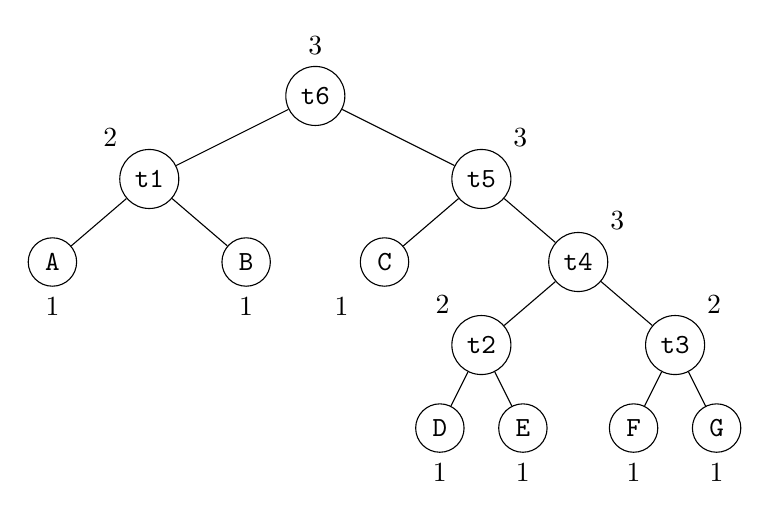
\begin{tikzpicture}[
        level 1/.style = {sibling distance = 12em, level distance = 3em},
        level 2/.style = {sibling distance = 7em, level distance = 3em},
        level 3/.style = {sibling distance = 7em, level distance = 3em},
        level 4/.style = {sibling distance = 3em, level distance = 3em},
    ]
    \tikzstyle{treenode} = [circle, draw=black];
    \node [treenode] (t6) {\texttt{t6}}
        child {node [treenode] (t1) {\texttt{t1}}
            child {node [treenode] (A) {\texttt{A}}}
            child {node [treenode] (B) {\texttt{B}}}
        }
        child {node [treenode] (t5) {$\texttt{t5}$}
            child {node [treenode] (C) {\texttt{C}}}
            child {node [treenode] (t4) {\texttt{t4}}
                child {node [treenode] (t2) {\texttt{t2}}
                    child {node [treenode] (D) {\texttt{D}}}
                    child {node [treenode] (E) {\texttt{E}}}
                }
                child {node [treenode] (t3) {\texttt{t3}}
                    child {node [treenode] (F) {\texttt{F}}}
                    child {node [treenode] (G) {\texttt{G}}}
                }
            }
        };
    \node [above = 0.05em of t6] (et6) {3};
    \node [above right = 0.05em of t5] (et5) {3};
    \node [above right = 0.05em of t4] (et4) {3};
    \node [above right = 0.05em of t3] (et3) {2};
    \node [above left = 0.05em of t2] (et2) {2};
    \node [above left = 0.05em of t1] (et1) {2};
    \node [below = 0.05em of A] (eA) {1};
    \node [below = 0.05em of B] (eB) {1};
    \node [below left = 0.45em of C] (eC) {1};
    \node [below = 0.05em of D] (eD) {1};
    \node [below = 0.05em of E] (eE) {1};
    \node [below = 0.05em of F] (eF) {1};
    \node [below = 0.05em of G] (eG) {1};
    \end{tikzpicture}
\end{figure}
\subparagraph{2}
从根节点\texttt{t6}开始,生成表达式树优化代码,处理顺序及指令代码在树中的位置如图所示
\begin{figure}[H]
    \centering
    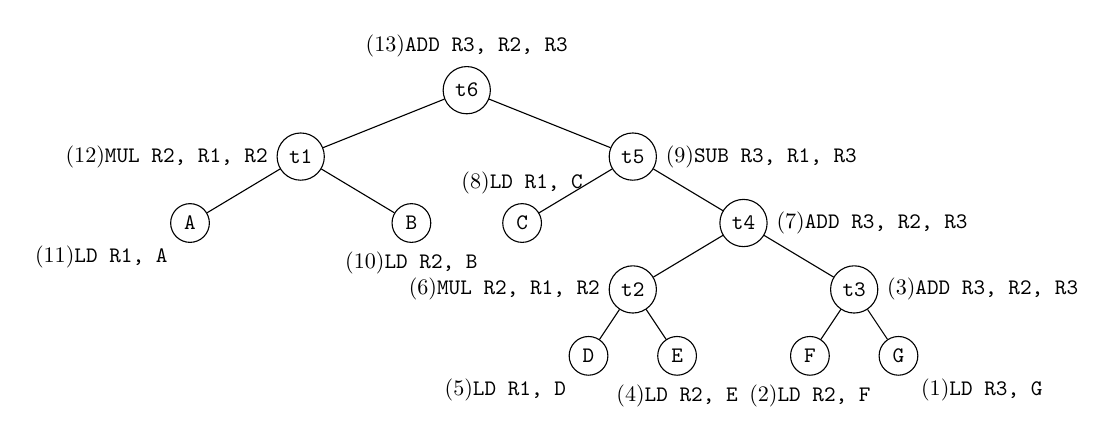
\begin{tikzpicture}[
        level 1/.style = {sibling distance = 15em, level distance = 3em},
        level 2/.style = {sibling distance = 10em, level distance = 3em},
        level 3/.style = {sibling distance = 10em, level distance = 3em},
        level 4/.style = {sibling distance = 4em, level distance = 3em},
        scale = 0.8,
        transform shape
    ]
    \tikzstyle{treenode} = [circle, draw=black];
    \node [treenode] (t6) {\texttt{t6}}
        child {node [treenode] (t1) {\texttt{t1}}
            child {node [treenode] (A) {\texttt{A}}}
            child {node [treenode] (B) {\texttt{B}}}
        }
        child {node [treenode] (t5) {$\texttt{t5}$}
            child {node [treenode] (C) {\texttt{C}}}
            child {node [treenode] (t4) {\texttt{t4}}
                child {node [treenode] (t2) {\texttt{t2}}
                    child {node [treenode] (D) {\texttt{D}}}
                    child {node [treenode] (E) {\texttt{E}}}
                }
                child {node [treenode] (t3) {\texttt{t3}}
                    child {node [treenode] (F) {\texttt{F}}}
                    child {node [treenode] (G) {\texttt{G}}}
                }
            }
        };
    \node [above = 0.05em of t6] (et6) {(13)\texttt{ADD R3, R2, R3}};
    \node [right = 0.05em of t5] (et5) {(9)\texttt{SUB R3, R1, R3}};
    \node [right = 0.05em of t4] (et4) {(7)\texttt{ADD R3, R2, R3}};
    \node [right = 0.05em of t3] (et3) {(3)\texttt{ADD R3, R2, R3}};
    \node [left = 0.05em of t2] (et2) {(6)\texttt{MUL R2, R1, R2}};
    \node [left = 0.05em of t1] (et1) {(12)\texttt{MUL R2, R1, R2}};
    \node [below left = 0.05em of A] (eA) {(11)\texttt{LD R1, A}};
    \node [below = 0.05em of B] (eB) {(10)\texttt{LD R2, B}};
    \node [above = 0.05em of C] (eC) {(8)\texttt{LD R1, C}};
    \node [below left = 0.05em of D] (eD) {(5)\texttt{LD R1, D}};
    \node [below = 0.05em of E] (eE) {(4)\texttt{LD R2, E}};
    \node [below = 0.05em of F] (eF) {(2)\texttt{LD R2, F}};
    \node [below right = 0.05em of G] (eG) {(1)\texttt{LD R3, G}};
    \end{tikzpicture}
\end{figure}
整理得到目标代码序列如下
\begin{lstlisting}[style = Assembler, alsolanguage = C]
    LD R3, G
    LD R2, F
    ADD R3, R2, R3
    LD R2, E
    LD R1, D
    MUL R2, R1, R2
    ADD R3, R2, R3
    LD R1, C
    SUB R3, R1, R3
    LD R2, B
    LD R1, A
    MUL R2, R1, R2
    ADD R3, R2, R3
\end{lstlisting}
\subparagraph{3}
在2个寄存器可用时,自底向上计算得到各个结点的代价数组,得到该表达式树的最优计算路径如图所示。(结点标号从小到大)

\begin{figure}[H]
    \centering
    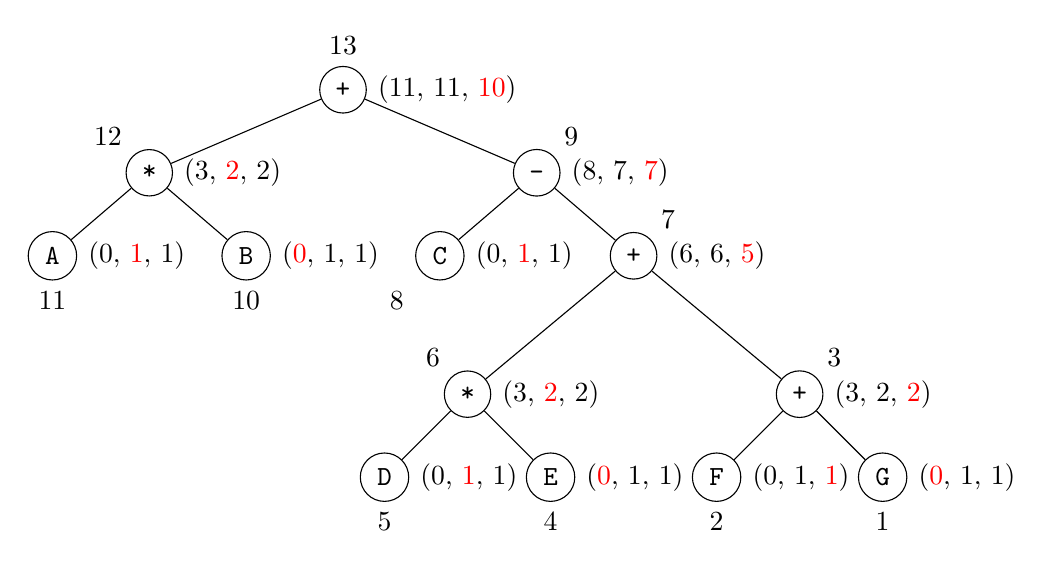
\begin{tikzpicture}[
        level 1/.style = {sibling distance = 14em, level distance = 3em},
        level 2/.style = {sibling distance = 7em, level distance = 3em},
        level 3/.style = {sibling distance = 12em, level distance = 5em},
        level 4/.style = {sibling distance = 6em, level distance = 3em},
    ]
    \tikzstyle{treenode} = [circle, draw=black];
    \node [treenode] (t6) {\texttt{+}}
        child {node [treenode] (t1) {\texttt{*}}
            child {node [treenode] (A) {\texttt{A}}}
            child {node [treenode] (B) {\texttt{B}}}
        }
        child {node [treenode] (t5) {$\texttt{-}$}
            child {node [treenode] (C) {\texttt{C}}}
            child {node [treenode] (t4) {\texttt{+}}
                child {node [treenode] (t2) {\texttt{*}}
                    child {node [treenode] (D) {\texttt{D}}}
                    child {node [treenode] (E) {\texttt{E}}}
                }
                child {node [treenode] (t3) {\texttt{+}}
                    child {node [treenode] (F) {\texttt{F}}}
                    child {node [treenode] (G) {\texttt{G}}}
                }
            }
        };
    \node [right = 0.05em of t6] (arrayt6) {(11, 11, {\color{red} 10})};
    \node [right = 0.05em of t5] (arrayt5) {(8, 7, {\color{red} 7})};
    \node [right = 0.05em of t4] (arrayt4) {(6, 6, {\color{red} 5})};
    \node [right = 0.05em of t3] (arrayt3) {(3, 2, {\color{red} 2})};
    \node [right = 0.05em of t2] (arrayt2) {(3, {\color{red} 2}, 2)};
    \node [right = 0.05em of t1] (arrayt1) {(3, {\color{red} 2}, 2)};
    \node [right = 0.05em of A] (arrayA) {(0, {\color{red} 1}, 1)};
    \node [right = 0.05em of B] (arrayB) {({\color{red} 0}, 1, 1)};
    \node [right = 0.05em of C] (arrayC) {(0, {\color{red} 1}, 1)};
    \node [right = 0.05em of D] (arrayD) {(0, {\color{red} 1}, 1)};
    \node [right = 0.05em of E] (arrayE) {({\color{red} 0}, 1, 1)};
    \node [right = 0.05em of F] (arrayF) {(0, 1, {\color{red} 1})};
    \node [right = 0.05em of G] (arrayG) {({\color{red} 0}, 1, 1)};
    \node [above = 0.05em of t6] (et6) {13};
    \node [above right = 0.05em of t5] (et5) {9};
    \node [above right = 0.05em of t4] (et4) {7};
    \node [above right = 0.05em of t3] (et3) {3};
    \node [above left = 0.05em of t2] (et2) {6};
    \node [above left = 0.05em of t1] (et1) {12};
    \node [below = 0.05em of A] (eA) {11};
    \node [below = 0.05em of B] (eB) {10};
    \node [below left = 0.45em of C] (eC) {8};
    \node [below = 0.05em of D] (eD) {5};
    \node [below = 0.05em of E] (eE) {4};
    \node [below = 0.05em of F] (eF) {2};
    \node [below = 0.05em of G] (eG) {1};
    \end{tikzpicture}
\end{figure}
最优代码序列是
\begin{lstlisting}[style = Assembler, alsolanguage = C]
    LD R1, F
    ADD R1, R1, G
    LD R0, D
    MUL R0, R0, E
    ADD R1, R0, R1
    LD R0, C
    SUB R1, R0, R1
    LD R0, A
    MUL R0, R0, B
    ADD R1, R1, R0
\end{lstlisting}
\end{document}

